\subsection{Website}
\begin{frame}
    \begin{columns}
	\begin{column}
	    {0.4\textwidth}
	    {\color{darkblue} http://pseudopotentiallibrary.org}
	    \scriptsize
	    \begin{itemize}
		\item[] Updated as new correlated ECPs are developed
		\item[]
		\item[] Anyone can contribute ECPs through \url{http://github.com/QMCPACK/pseudopotentiallibrary}
		\item[]
		\item[] Soon will include completed table up through Kr
		\item[]
        \item[] KB projectors for {\it some} atoms are available, will update as they become available
	    \end{itemize}
	\end{column}
	\begin{column}
	    {0.6\textwidth}
	    \begin{figure}[h]
		\centering
		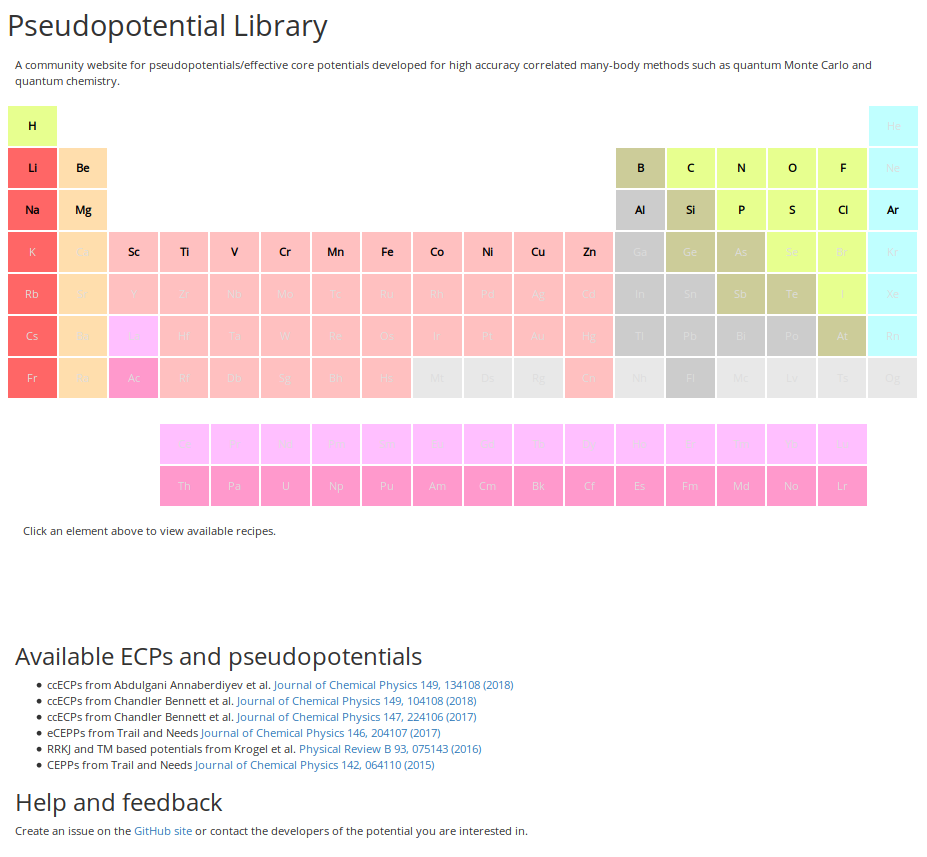
\includegraphics[width=0.8\textwidth]{figures/pseudopotentiallibrary}
	    \end{figure}
	\end{column}
    \end{columns}
\end{frame}

\begin{frame}
    \begin{columns}
	\begin{column}
	    {0.3\textwidth}
        {\color{wolfred} ccECP format} 
        \tiny
            \hfil $V_\ell(r) = \sum\limits_{k=1}^{N_\ell} \beta_k r^{n_k-2} e^{-\alpha_k r^2}$
        \begin{eqnarray*}
            \begin{array}{ccc}
                Z_{\rm eff} & L+1 \\
                N_0 & \ldots & N_{L} 
            \end{array}\\
            \left.
            \begin{array}{ccc}
                n_1 & \alpha_1 & \beta_1 \\
                \vdots & \vdots & \vdots \\
                n_{N_0} & \alpha_{N_0} & \beta_{N_0}
            \end{array}\right\} \ell=0 \\
            \begin{array}{ccc}
                & \vdots 
            \end{array}\\
            \left.
            \begin{array}{ccc}
                    n_1 & \alpha_1 & \beta_1 \\
                    \vdots & \vdots & \vdots \\
                    n_{N_L} & \alpha_{N_L} & \beta_{N_L}
            \end{array}\right\} \ell=L
        \end{eqnarray*}
        {\normalsize \color{darkblue} Carbon Example}
        \lstinputlisting{C.ccECP}
	\end{column}
	\begin{column}
	    {0.7\textwidth}
	    %\begin{figure}[h]
		%\centering
		%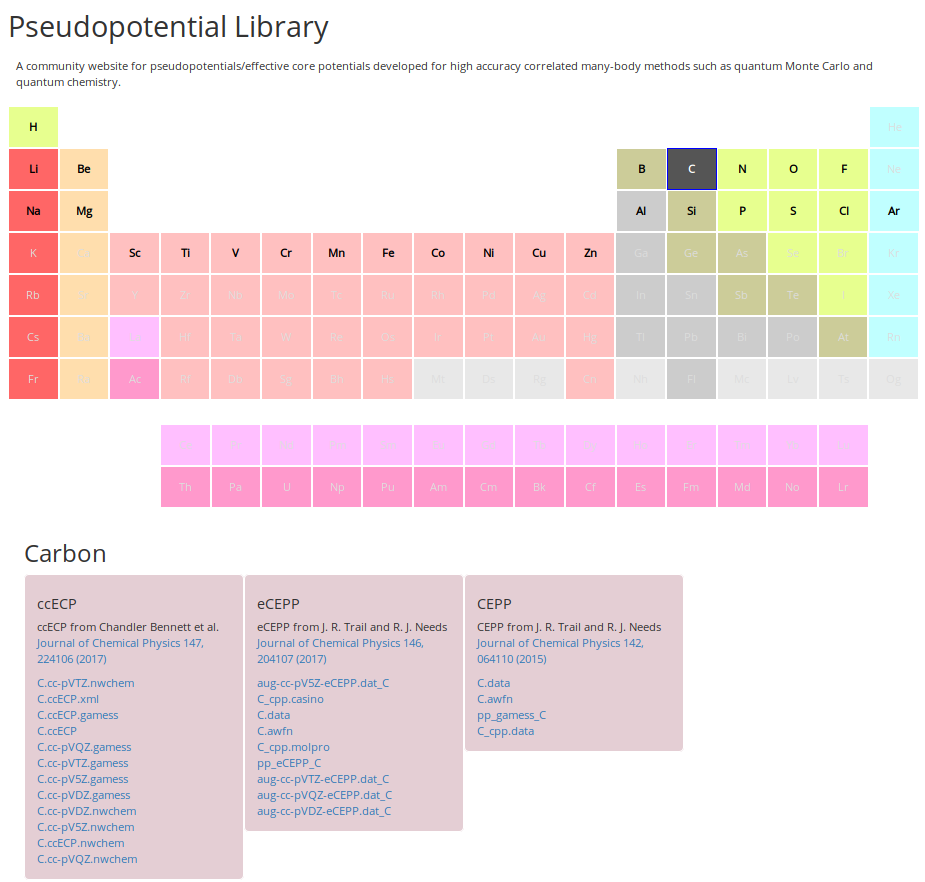
\includegraphics[width=0.8\textwidth]{figures/carbon-web}
	    %\end{figure}
		\begin{tikzpicture}
            \node [anchor=west] (water) at (-1,1.2) {\footnotesize C.ccECP};
		\begin{scope}[xshift=1.5cm]
		    \node[anchor=south west,inner sep=0] (image) at (0,0) {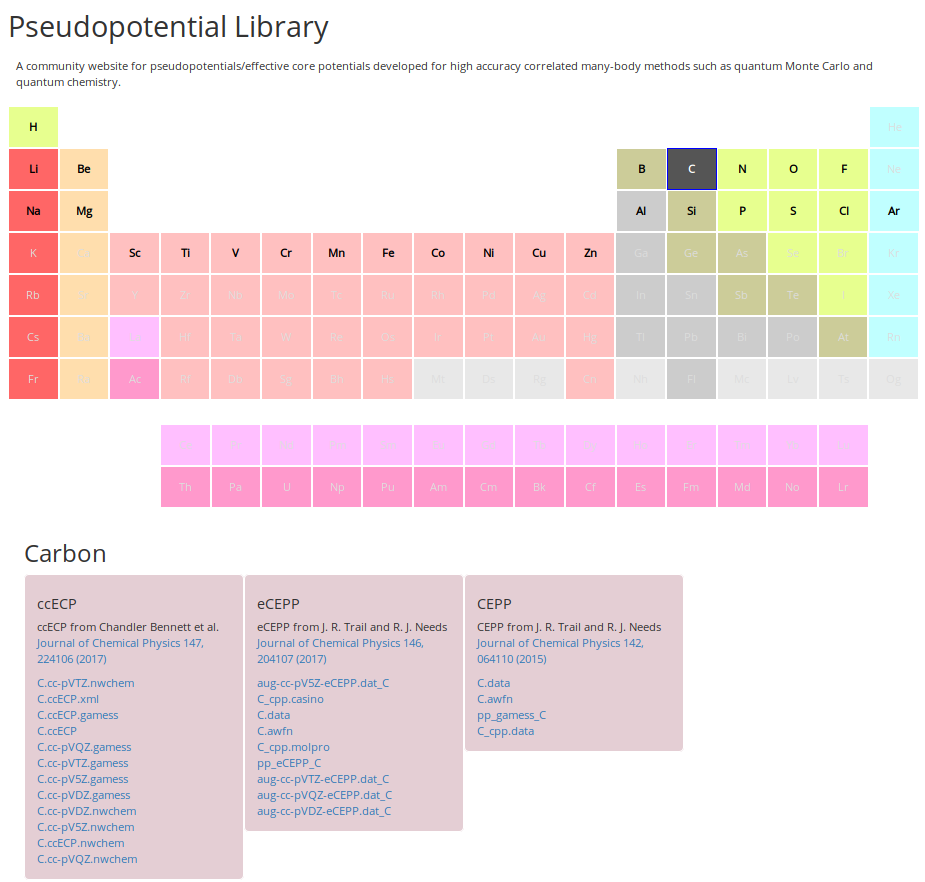
\includegraphics[width=0.7\textwidth]{figures/carbon-web}};
		    \begin{scope}[x={(image.south east)},y={(image.north west)}]
		        \draw [-stealth, line width=1pt, wolfred] (water) -- ++(0.24,0.0);
		    \end{scope}
		\end{scope}
		\end{tikzpicture}%
	\end{column}
    \end{columns}
\end{frame}

\begin{frame}
    {Available Quantum Chemistry Formats}
    For each ccECP, we include a variety of basis sets and pseudopotential formats for various codes, including cc-pV$n$Z and aug-cc-pV$n$Z basis sets, with $n \in \{\rm D,T,Q,5\}$.\\
    \bigskip
    Basis/ECP formats included for each code QMCPACK interfaces to
    \begin{enumerate}
        \item[] \textsc{\color{ForestGreen}GAMESS}: Basis sets and pseudopotential format\\
            {\hfil e.g. {\color{NavyBlue} C.cc-pVTZ.gamess \& C.ccECP.gamess}}
        \item[] \textsc{\color{Plum}Quantum Package}: Uses \textsc{GAMESS} file formats\\
            {\hfil e.g. {\color{NavyBlue} C.cc-pVTZ.gamess \& C.ccECP.gamess}}
        \item[] \textsc{\color{RedOrange}PySCF}: Parses \textsc{NWChem} formats\\
            {\hfil e.g. {\color{NavyBlue} C.cc-pVTZ.nwchem \& C.ccECP.nwchem}}
        \item[] \textsc{\color{wolfred}Qmcpack}: Uses qmcpack xml format\\
            {\hfil e.g. {\color{NavyBlue} C.ccECP.xml}}
    \end{enumerate}
\end{frame}

\subsection{Example}
\begin{frame}
    {PySCF Example: Catom.py}
    \small
    \lstset{language=Python,basicstyle=\ttfamily,keywordstyle=\color{blue}\ttfamily,commentstyle=\color{ForestGreen}\ttfamily,stringstyle=\color{red}\ttfamily,showstringspaces=false}
    \only<1-1>{\lstinputlisting[firstline=1,lastline=9]  {../files/quantum_chemistry/Catom.py}}
    \only<2-2>{\lstinputlisting[firstline=11,lastline=24]{../files/quantum_chemistry/Catom.py}}
    \only<3-3>{\lstinputlisting[firstline=26,lastline=37]{../files/quantum_chemistry/Catom.py}}
    \only<4-4>{\lstinputlisting[firstline=38,lastline=48]{../files/quantum_chemistry/Catom.py}}
\end{frame}

